
\section{Разработанное решение}
\begin{figure}
  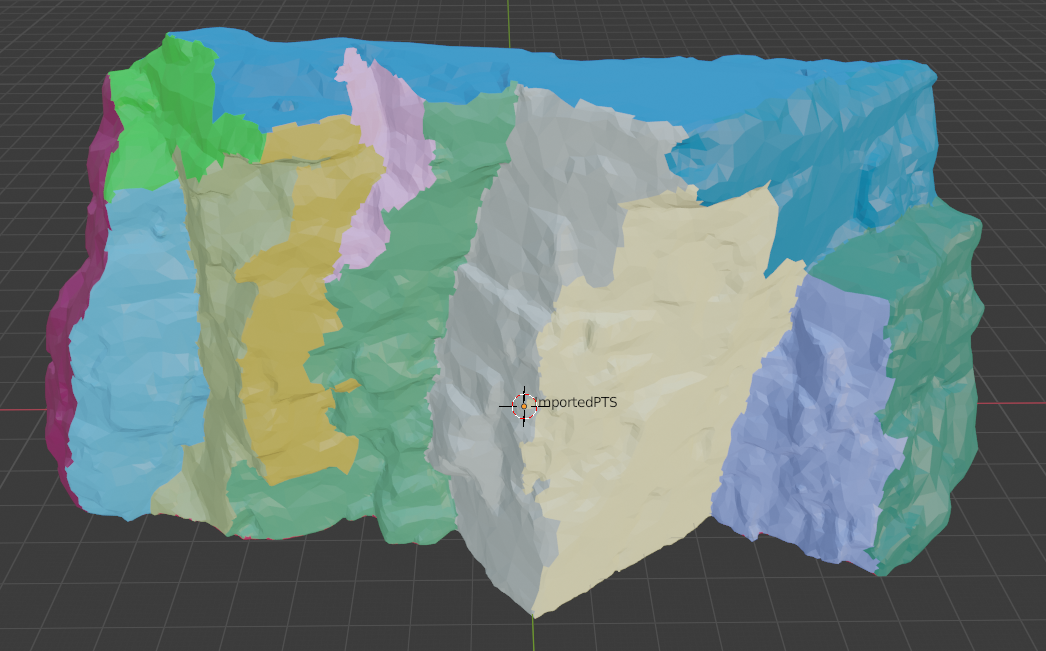
\includegraphics[scale=0.145]{clustering.png}
  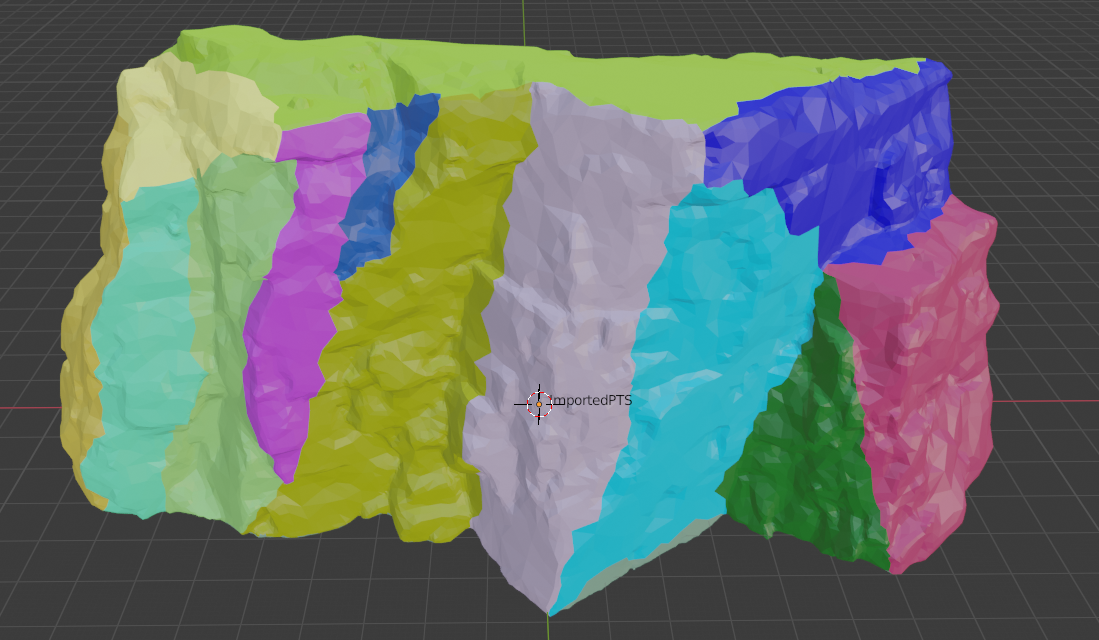
\includegraphics[scale=0.145]{straightening.png}
  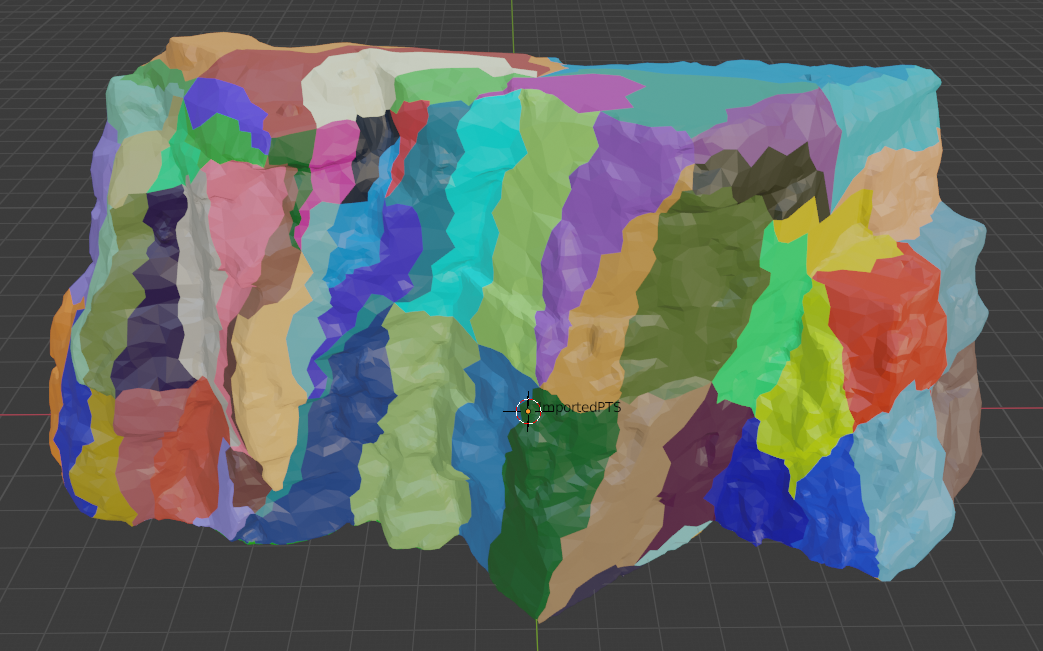
\includegraphics[scale=0.145]{quadrangulation.png}
  \caption{Визуализация этапа предобработки (слева направо: кластеризация, распрямление границ, квадрангуляция)}
\end{figure}

В базовом виде алгоритм из статьи \cite{niski2007multi} делится на два этапа: предобработка и рендеринг. Алгоритм предобработки принимает на вход дискретное многообразие (возможно с краем), хранимое в формате ``треугольного супа'' -- неиндексированного набора треугольников, где каждый треугольник задан аттрибутами его вершин. Этот формат был выбран в целях упрощения имплементации предобработки во внешней памяти.

\subsection{Предобработка}
Цель этапа предобработки -- построить непрерывный атлас меша, а затем ресемплировать атрибуты в каждой карте атласа по равномерной сетке в параметрическом пространстве, тем самым получив семейство геометрических изображений. Предлагаемый алгоритм состоит из следующих этапов:
\begin{enumerate}
\item Раскладывание треугольников по бакетам
\item Кластеризация треугольников в рамках бакетов
\item Глобальная кластеризация
\item Распрямление границ кластеров
\item Квадрангуляция
\item Репараметризация
\item Ресемплинг
\end{enumerate}

\subsubsection{Раскладывание треугольников по бакетам}
Этот и последующий этапы фактически являются оптимизациями основного алгоритма, необходимыми для работы с большими мешами. Пространство модели разбивается по прямоугольной равномерной трёхмерной сетке на ``бакеты'', треугольники каждого бакета проходят следующий этап независимо, что позволяет запускать его параллельно на многоядерных процессорах.

\subsubsection{Кластеризация}
Цель кластеризации -- разбить все треугольники на непересекающиеся связные множества (называемые кластерами), оптимизируя некоторые эвристики и сохраняя некоторые инварианты. В данной работе используются эвристики планарности, компактности и изменения иррегулярности. Новые кластеры строятся последовательным объединением имеющихся кластеров минимизируя целевые эвристики.

Пусть $M$ -- кластер, состоящий из вершин $\{v_1, ..., v_k\}$. Для удобства будем считать, что вершины заданы в однородных координатах. Плоскость будем задавать однородным вектором $n$, задающим множество точек плоскости как решения $n^\top v = 0$. Рассмотрим среднеквадратичное отклонение вершин кластера от произвольной поверхности:
\[
  E_M(n) = \frac{1}{k}\sum_{i=1}^k (n^\top v_i)^2.
\]
Обозначим точку минимума этой функции, то есть прямую приближающую кластер методом наименьших квадратов, за $n_0$. Тогда эвристикой планарности кластера назовём
\[
  E_{fit}(M) = E_M(n_0).
\]
Конечно же вычисление этой эвристики заново на каждой итерации алгоритма приведёт к квадратичной асимптотике, что неудовлетворительно. Для эффективного вычисления в \cite{garland2001} предлагается использовать поверхности второго порядка. Раскрывая скобки в определении $E_M$,
\[
  E_M(n) = \frac{1}{k}\sum_{i=1}^k n^\top(v_iv_i^\top) n
    = \frac{1}{k}n^\top\left(\sum_{i=1}^k v_iv_i^\top\right) n
    = \frac{1}{k}n^\top Q_M n,
\]
где $Q_M = \sum_{i=1}^k v_iv_i^\top$. Так как $Q_{M\cup N} = Q_M + Q_N$, для вычисления $E_M$ достаточно хранить для каждого кластера его форму $Q_M$, а при объединении кластеров складывать их.

Саму МНК плоскость можно найти используя выборочную ковариационную матрицу
\[
  Z = \frac{1}{1-k}\sum_{i=1}^k (v_i - \bar v)(v_i - \bar v)^\top.
\]
Первые три координаты $n_0$ будут равны первым трём координатам собственного вектора $Z$ соответствующего наименьшему собственному значению, а последняя координата может быть вычислена из равенства $n_0^\top \bar v = 0$. К счастью, матрица $Z$ также может быть вычислена через форму $Q_M$:
\[
  Z = \sum_{i=1}^k v_iv_i^\top - k(\bar v \bar v^\top) = Q_M - \frac{Q_{M1:3,4}Q_{M1:3,4}^\top}{Q_{M4,4}},
\]
где константа пропорциональности опущена так как не влияет на направления собственных векторов и положения в вариационном ряду собственных значений. Это наблюдение и позволяет вычислять ошибку планарности на каждой итерации алгоритма за $O(1)$.

Пусть площадь и периметр кластера $M$ равны $A$ и $P$ соответственно. Тогда иррегулярностью кластера называют величину
\[
  \gamma(M) = \frac{P^2}{4\pi A}.
\]
Иррегулярность измеряет степень схожести кластера с диском. Эвристикой изменения иррегулярности для объединения кластеров $N_1, N_2$ в кластер $M$ называют
\[
  E_{shape} = \frac{\gamma(M) - \max(\gamma(N_1), \gamma(N_2))}{\gamma(M)}.
\]
Эвристикой компактности же назовём
\[
  E_{comp}(M) = P^2.
\]

Эвристики изменения иррегулярности и планарности взяты из работы \cite{garland2001}, но попытка использовать подход описанный в этой работе как есть не увенчалась успехом: эвристика ориентации не вносила значительного вклада в результат на тестовых моделях, а эвристики изменения иррегулярности оказалось недостаточно чтобы предать кластерам округлую форму (отношение квадрата периметра к площади кластера могло оставаться близким к $4\pi$ даже когда кластер имеет крайне вытянутую форму за счёт ``ребристости'' поверхности, так как ребристость увеличивает площадь не меняя периметра). Было принято решение отказаться от эвристики ориентации, а эвристику изменения иррегулярности заменить на некоторую другую метрику. Из вариантов были рассмотрены просто иррегулярность, квадрат периметра и сумма квадрата периметра и изменения иррегулярности. Последний вариант дал наиболее благоприятный результат: сам по себе квадрат периметра приводил к слишком ломаным границам между кластерами, а учёт изменения иррегулярности позволил сгладить этот эффект. Однако квадрат периметра не совпадает по размерности с остальными эвристиками, что потребовало подбора коэффициента вклада этой эвристики под конкретную модель. На использованных тестовых моделях (ландшафты \cite{quixel_megascans}) наилучший результат дал коэффициент $10^{-4}$ для компактности, $1.7$ для планарности и $1$ для изменения иррегулярности.

В процессе кластеризации на кластеры накладывается следующий топологический инвариант: пересечение любых двух кластеров гомеоморфно либо точке, либо отрезку, и при этом граница любого кластера гомеоморфна окружности. Этот инвариант позволит на этапе квадрангуляции получить разбиение, удовлетворяющее определению непрерывного атласа.

Используется жадный алгоритм кластеризации, строящий кластеры снизу-вверх. Поддерживается очередь с приоритетами из пар кластеров -- претендентов на слияние. Приоритетом является сумма эвристик посчитанных для объединения кластеров. В ходе итерации алгоритм берёт потенциальный мердж с минимальной ошибкой из очереди, проверяет не нарушит ли он топологические инварианты, объединяет кластеры с использованием структуры данных ``система непересекающихся множеств'', затем обновляет приоритеты потенциальных мерджей кластера этой итерации и его соседей. Алгоритм прекращает свою работу при достижении целевого количества кластеров или превышении дозволенной ошибки.

\subsubsection{Глобальная и локальная кластеризация}
\begin{figure}[ht]
\minipage{0.32\textwidth}
  \centering
  \begin{tikzpicture}[scale=1.2]
    \coordinate (A) at (0,1.5);
    \coordinate (B) at (0,1);
    \coordinate (C) at (0,-1);
    \coordinate (D) at (0,-1.5);

    \filldraw[blue!10] (-2, 2) -- (-0.5, 2) -- (A) -- (B) -- (-0.5,0) -- (C) -- (D) -- (-0.5,-2) -- (-2,-2) -- cycle;
    \filldraw[red!10] (2, 2) -- (-0.5, 2) -- (A) -- (B) -- (-0.5,0) -- (C) -- (D) -- (-0.5,-2) -- (2,-2) -- cycle;

    \draw (-0.5, 2) -- (A) -- (B) -- (-0.5,0) -- (C) -- (D) -- (-0.5,-2);
    \draw (2,2) -- (A) -- (B) -- (1,0) -- (C) -- (D) -- (2,-2);

    \node at (-1.5,0) {А};
    \node at (1.5,0) {Б};
  \end{tikzpicture}
  \caption{Нарушение инварианта при наивном объединении бакетов}
  \label{fig:naive_inv_invalid}
\endminipage\hfill
%
\minipage{0.32\textwidth}
  \centering
  \begin{tikzpicture}[scale=1.2]
    \coordinate (E) at (0.5,1.25);
    \coordinate (F) at (0.5,-1.25);
    \coordinate (O) at (1.25,-0.75);

    \filldraw[blue!10] (-2, 2) -- (-0.5, 2) -- (A) -- (B) -- (-0.5,0) -- (C) -- (D) -- (-0.5,-2) -- (-2,-2) -- cycle;
    \filldraw[red!10] (2,2) -- (1, 2) -- (E) -- (0.75,0) -- (1.25,-0.25) -- (1.75,-0.75) -- (1.25,-1.25) -- (F) -- (1,-2) -- (2,-2) -- cycle;


    \draw (-0.5, 2) -- (A) -- (B) -- (-0.5,0) -- (C) -- (D) -- (-0.5,-2);
    \draw (1, 2) -- (E) -- (0.75,0) -- (1.25,-0.25) -- (1.75,-0.75) -- (1.25,-1.25) -- (F) -- (1,-2);
    \draw (0.75,0) -- (-0.5,0) -- (F) -- cycle;

    \draw  (0.75,0) -- (O) -- (1.25,-0.25) -- (O) -- (1.75,-0.75) -- (O) -- (1.25,-1.25) -- (O) -- (F);

    \node at (0.25,-0.4) {А};
    \node at (1.5,0) {Б};
  \end{tikzpicture}
  \caption{Нарушение инварианта при объединении бакетов с разграничителем}
  \label{fig:smart_inv_invalid}
\endminipage\hfill
%
\minipage{0.32\textwidth}
  \centering
  \begin{tikzpicture}[scale=1.2]
    \filldraw[blue!10] (-2, 2) -- (-0.5, 2) -- (A) -- (B) -- (-0.5,0) -- (C) -- (D) -- (-0.5,-2) -- (-2,-2) -- cycle;
    \filldraw[red!10] (2,2) -- (1, 2) -- (E) -- (0.75,0) -- (1.25,-0.25) -- (1.75,-0.75) -- (1.25,-1.25) -- (F) -- (1,-2) -- (2,-2) -- cycle;


    \draw (-0.5, 2) -- (A) -- (B) -- (-0.5,0) -- (C) -- (D) -- (-0.5,-2);
    \draw (1, 2) -- (E) -- (0.75,0) -- (1.25,-0.25) -- (1.75,-0.75) -- (1.25,-1.25) -- (F) -- (1,-2);
    \draw (0.75,0) -- (-0.5,0) -- (F) -- cycle;

    \draw  (0.75,0) -- (O) -- (1.25,-0.25) -- (O) -- (1.75,-0.75) -- (O) -- (1.25,-1.25) -- (O) -- (F);

    \draw[red] (-0.5,0) -- (0.625,-0.625) -- (O);
    \filldraw[red] (0.625,-0.625) circle (2pt);
  \end{tikzpicture}
  \caption{Устранение нарушений при объединении бакетов с разграничителями}
  \label{fig:inv_valid}
\endminipage\hfill
\end{figure}
Приведённый алгоритм кластеризации используется и на 3 и на 4 этапах, но в ходе 3 этапа каждый треугольник в бакете считается отдельным кластером, а в ходе 4 этапа изначальным набором кластеров берётся объединение результатов работы предыдущего этапа. Очевидно, на входе 3 этапа топологический инвариант выполнен. Каждая итерация алгоритма сохраняет инвариант, поэтому в рамках каждого бакета он тоже выполнен. Однако несложно построить пример ситуации когда инвариант нарушается при объединении бакетов. На рисунке  \ref{fig:naive_inv_invalid} синим и красным цветом обозначены кластеры двух разных бакетов соответственно. Кластеры А и Б пересекаются по несвязному множеству, тем самым нарушая инвариант, хотя в рамках каждого бакета инвариант выполнен. В работе \cite{niski2007multi} никак не уточняется этот момент, однако практика показывает что если бакеты достаточно велики отностельно детализации меша, то эта проблема возникает достаточно редко. С целью устранения этой проблемы было решено не включать в бакет треугольники пересекающие его границы, а добавлять их как отдельные кластеры при переходе к 4 этапу. Этот подход позволяет частично избежать ситуации с рисунка \ref{fig:naive_inv_invalid}, но инвариант всё ещё может быть нарушен как на рисунке \ref{fig:smart_inv_invalid}: кластер границы А и кластер правого бакета Б пересеклись по несвязному множеству, двум точкам. Если в дополнение к этому подходу разделять треугольники нарушившие инвариант на 2 части, либо использовать граничные треугольники в проверке инварианта в каждом бакете, то проблема окончательно пропадает. В данной работе был выбран следующий подход. Рассмотрим множество треугольников, пересёкших границы бакетов (то есть таких, что не все вершины попали в один бакет. Это условие необходимо и достаточно, так как и треугольник и бакет -- выпуклые множества). Ясно, что топологически эта фигура является двумерной поверхность с $n$ дырками. Обозначим за $A_i$ множества вершин, образующие границы дырок. Рассмотрим такие рёбра, что их вершины принадлежат множеству $A_i$, но на ребро опираются 2 треугольника (т.е. ребро не лежит на границе дырки). Разделим все такие рёбра и смежные с ними треугольники пополам (рисунок \ref{fig:inv_valid}). Легко понять, что после этой операции любой треугольник пересекается со всей поверхностью кластера либо ровно по одной вершине, либо ровно по одному ребру, чего и достаточно для соблюдения инварианта при объединении всех бакетов и граничного множества.

\begin{figure}[ht]
\centering
\begin{tikzpicture}
  \filldraw[blue!10] (-4,0) -- (-3,1) -- (-2,0.75) -- (-1,1.25) -- (1,0.5) -- (3,2) --
    (4,0) -- (3,-1) -- (1,-0.5) -- (-1,-1.5) -- (-2.5,-1) -- cycle;
  \draw[very thick] (-4,0) -- (-3,1) -- (-2,0.75) -- (-1,1.25) -- (1,0.5) -- (3,2) --
    (4,0) -- (3,-1) -- (1,-0.5) -- (-1,-1.5) -- (-2.5,-1) -- cycle;
  \draw (-2,0.75) -- (-1,-1.5);
  \draw (1,0.5) -- (1,-0.5);

  \draw[red, thick] (-2,0.75) -- (-1,1.25) -- (1,0.5);
  \draw[red, thick] (1,-0.5) -- (-1,-1.5);
  \node at (-0.5,0) {А};
\end{tikzpicture}
\caption{Атлас с картой А пересекающей границу по несвязному множеству (отмечено красным)}
\label{fig:weird_edge}
\end{figure}
Ещё одним тонким моментом в процессе кластеризации является работаа с границей многообразия. Авторы \cite{purnomo2004} не уточняют в своих определениях считается ли атлас, одна из карт которого имеет область определения пересекающуюся с границей меша по двум несвязным отрезкам, корректным (рисунок \ref{fig:weird_edge}). В данной работе считается, что вся граница многообразия является границей одной мнимой карты, что запрещает ситуации как на рисунке.

\subsubsection{Распрямление границ}
При использовании некоторых эвристик границы кластеров получаются достаточно ломанными, что приводит к артефактам на их границах при рендеринге. С целью борьбы с этой проблемой на этом этапе пары граничащих кластеров загружаются в память и граница между ними заменяется на кратчайший путь из конца в начало найденный алгоритмом Дейкстры \cite{dijkstra}. В этот этап тоже достаточно легко вносится параллелизм. Так как операция распрямления границы мутирует пару файлов-кластеров, необходимо лишь убедится что никакие два исполнителя не будут параллельно распрямлять границы принадлежащие одному кластеру.

\subsubsection{Квадрангуляция}
\begin{figure}[ht]
\minipage{0.475\textwidth}
  \centering
  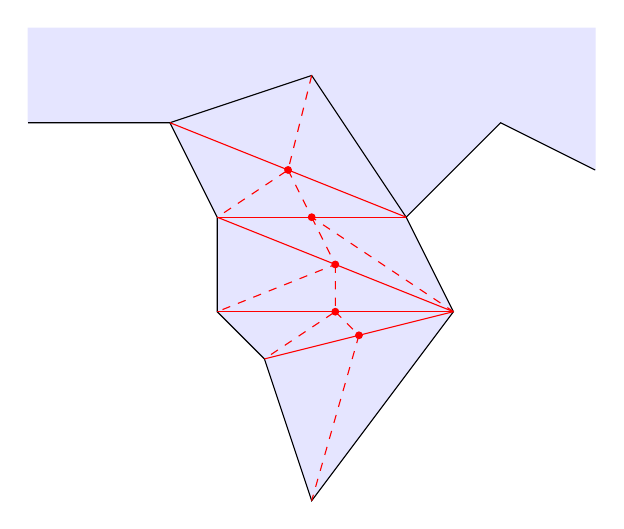
\begin{tikzpicture}[scale=1.2]
    \filldraw[blue!10] (-3,1) -- (-3,0)
    -- (-1.5,0) -- (-1,-1) -- (-1,-2) -- (-0.5,-2.5)
    -- (0,-4)
    -- (1.5,-2) -- (1,-1)
    -- (2,0) -- (3,-0.5) -- (3,1) -- cycle;

    \draw (-3,0)
    -- (-1.5,0) -- (-1,-1) -- (-1,-2) -- (-0.5,-2.5)
    -- (0,-4)
    -- (1.5,-2) -- (1,-1)
    -- (2,0) -- (3,-0.5);
    \draw (-1.5,0) -- (0,0.5) -- (1,-1);

    \draw[red] (-1.5,0) -- (1,-1);
    \draw[red] (1,-1) -- (-1,-1);
    \draw[red] (-1,-1) -- (1.5,-2);
    \draw[red] (1.5,-2) -- (-1,-2);
    \draw[red] (1.5,-2) -- (-0.5,-2.5);

    \draw[dashed,red] (0,0.5) -- (-0.25,-0.5) -- (-1,-1);
    \draw[dashed,red] (-0.25,-0.5) -- (0,-1) -- (1.5,-2);
    \draw[dashed,red] (0,-1) -- (0.25,-1.5) -- (-1,-2);
    \draw[dashed,red] (0.25,-1.5) -- (0.25,-2) -- (-0.5,-2.5);
    \draw[dashed,red] (0.25,-2) -- (0.5,-2.25) -- (0,-4);

    \filldraw[red] (-0.25,-0.5) circle (1pt);
    \filldraw[red] (0,-1) circle (1pt);
    \filldraw[red] (0.25,-1.5) circle (1pt);
    \filldraw[red] (0.25,-2) circle (1pt);
    \filldraw[red] (0.5,-2.25) circle (1pt);
  \end{tikzpicture}
  \caption{Разделение рёбер для построения путей при квадранугялции. Сплошные красные -- рёбра, подлежащие разделению, красные точки -- новые вершины, красный пунктир -- дополнительные рёбра}
  \label{fig:quadr_split}
\endminipage\hfill
%
\minipage{0.475\textwidth}
  \centering
  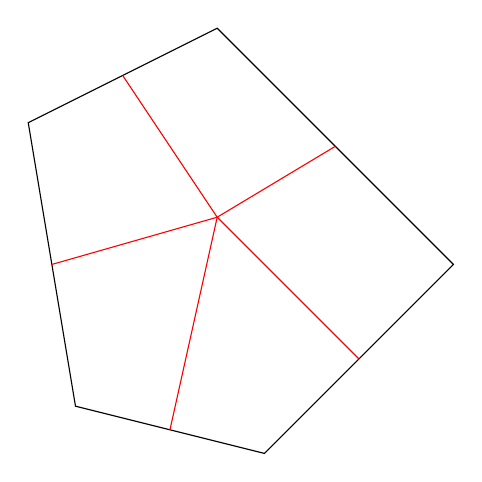
\begin{tikzpicture}[scale=1.2]
    \draw (-2,2) -- (0,3) -- (2.5,0.5) -- (0.5,-1.5) -- (-1.5,-1) -- cycle;
    \draw[red] (0,1) -- (-1,2.5);
    \draw[red] (0,1) -- (1.25,1.75);
    \draw[red] (0,1) -- (1.5,-0.5);
    \draw[red] (0,1) -- (-0.5,-1.25);
    \draw[red] (0,1) -- (-1.75,0.5);
  \end{tikzpicture}
  \caption{Квадрангуляция. Чёрные рёбра -- схематичное представление исходного кластера как многоугольника, красным -- пути разрезания кластера на четырёхугольники}
  \label{fig:quadr}
\endminipage
\end{figure}
Легко увидеть, что в результате кластеризации каждый кластер геометрически является $n$-угольником. Вершинами многоугольника назовём точки, в которых пересекаются более чем $2$ кластера, считая воображаемую область за границей меша отдельным кластером. Рёбрами назовём множества из тех точек, в которых пересекаются ровно 2 кластера. В ходе этого этапа в каждом кластере выделяется вершина меша, называемая центром, а затем проводятся кривые из центра к серединам рёбер. Кривые строятся алгоритмом $A^*$ \cite{astar} так, чтобы кривые шли как можно дальше друг от друга, от границы всего кластера, и не пересекались. Для достижения этого эффекта веса рёбер взвешиваются единицей делённой на расстоянием до нежелаемого множества. Порядок выбора рёбер для проведения кривых следующий: первая кривая произвольная, а затем в самом большом по количеству рёбер регионе из получившегося разбиения выбирается центральное ребро. Этот подход позволяет итоговым четырёхугольникам быть примерно одинакового масштаба и пропорций. В случае если это построение не возможно, предлагается разделять мешающие треугольники. Авторы не уточняют используемый алгоритм поиска мешающих треугольников, а также способ разделения, поэтому в данной работе было решено использовать следующий подход. На каждой итерации проведения кривой в регионе, ищутся все рёбра такие, что само ребро не лежит на границе, но при этом обе его вершины лежат на границе. Далее эти рёбра делятся пополам, как и опирающиеся на них треугольники. На рисунке \ref{fig:quadr_split} красным цветом обозначены описанные рёбра, а пунктиром обозначено дополнительное построение, получающееся в результате последовательного разделения красных рёбер. После этого разделения пути гарантированно будут существовать.

Пусть дан граф триангуляции диска, вершины $O$, $M$ лежат на границе, и любой путь между ними проходит ещё хотя бы один раз по границе. Покажем, что тогда найдётся ребро, не лежащее на границе, но обе вершины которого лежат на ней (назовём такие рёбра плохими). Тогда по контрапозиции получим корректность алгоритма.
%
Доказывать будем по индукции. Базой будут такие графы, в которых нет смежных внутренних вершин. Если же в графе есть смежные внутренние вершины, стянем ребро между ними. Каждому пути в старом графе можно сопоставить путь в новом графе, при этом не потеряв посещения границы на них. Значит по предположению индукции в графе есть плохое ребро. Но операция стягивания ребра не могла добавить новых плохих рёбер. Значит плохое ребро было и в старом графе.
%
Пусть в графе нет смежных внутренних вершин. Если в графе любая граничная вершина имеет степень не больше трёх, очевидно граф выглядит как $n$-угольник и в нём есть пути из любой вершины границы в любую другую не проходящие по границе, что противоречит условию. Значит найдётся вершина на границе со степенью хотя бы 4. Рассмотрим её соседей в порядке обхода. Заметим, что 2 подряд идущих соседа не могут быть внутренними вершинами. Значит кроме первой и последней вершины в порядке обхода мы нейдём ещё одну вершину лежащую на границе. Эта вершина и изначальная и будут образовывать целевое плохое ребро.
%
Таким образом в любом графе с описанными свойствами найдётся плохое ребро, что и требовалось доказать.

Из рисунка \ref{fig:quadr} видно, что в ходе этой операции многогранник будет разбит на четырёхугольники. Более того, легко увидеть, что полученное разделение будет удовлетворять определению непрерывного атласа. Пары четырёхугольников полученных из одного кластера пересекаются по построению либо по общей вершине, либо по общему ребру. Сами кластеры из поддерживаемого инварианта пересекаются аналогичным образом. А так как новые вершины ставятся на серединах рёбер кластеров одинаковым образом, из чего четырёхугольники разных кластеров тоже пересекаются либо по общему ребру, либо по общей вершине.

Стратегия выбора центра, предлагаемая \cite{purnomo2004}, достаточно произвольна. Выбирается одно из рёбер многогранника, из его центра проводятся кривые в центры других рёбер, а затем центры проведённых кривых в порядке обхода принимаются за новый многогранник, у которого на 1 ребро меньше, после чего процедура запускается рекурсивно пока не останется вырожденного многогранника из меньше чем трёх точек, центр которого берётся за центр всего кластера.

Отметим, что в случае если в кластере все вершины лежат на границе, алгоритм не будет работать корректно, так как не удастся найти центр. Эту проблему не сложно решить добавив новую произвольную вершину, но в данной работе не возникло в этом нужды так как столь малые кластеры не удовлетворительны для дальнейшей работы метода, и алгоритм кластеризации не оставляет таких кластеров при должном критерии остановки.

\subsubsection{Репараметризация}
После этапа квадрангуляции меш разделён на области определения карт для итогового атласа. Далее необходимо построить согласованные гомеоморфизмы для каждого четырёхугольника на единичный квадрат, то есть построить параметризацию. Задача построения параметризации широко известна в области компьютерной графики, и к её решению было придумано много подходов. Большая часть из них берут за исходную параметризацию вложение Татта \cite{tutte1963}, а затем оптимизируют некоторый целевой функционал, не нарушающий инъективности исходной параметризации. В данном алгоритме важно, чтобы при ресемплинге частота дискретизации была пропорциональна кривизне исходной поверхности в каждой точке, поэтому был выбран подход из статьи \cite{sander2001}. Для корректности получившегося атласа в процессе построения параметризации вершины, соответствующие углам четырёхугольника, были закреплены на углах единичного квадрата, а вершины лежащие на границе были распределены по границам квадрата пропорционально длине рёбер, и также зафиксированы.

\subsubsection{Ресемплинг}
Цель ресемплинга -- построить геометрические изображения содержащие информацию об атрибутах меша в его точках, соответствующих точкам на равномерной прямоугольной сетке в пространстве параметризации. Заметим, что при таком построении для двух соседних карт их пересечение будет семплировано в оба геометрических изображения соответствующих этим картам. Таким образом, если спроецировать области геометрических текстур на исходную модель, соседние изображения будут иметь пересечение в $0.5$ пикселя. Для удобства построения квадродеревьев в следующем разделе в качестве частоты ширины и высоты геометрических изображений берутся исключительно числа вида $2^n + 1$.

Также для адаптивного рендеринга необходимо сгенерировать мип-уровни для итоговых геометрических текстур. Авторы статьи \cite{purnomo2004} предлагают использовать фильтрацию с достаточно сложной обработкой граничных случаев, однако так как каждый следующий мип-уровень в 4 раза меньше предыдущего, делать ресемплинг для каждого уровня заново занимает всего в $\approx1.3$ раза дольше ресемплинга самого высокочастотного мип-уровня, поэтому в данной работе был выбран именно этот подход.

Небольшой проблемой упомянутой в \cite{niski2007multi} стали правила растеризации. При семплировании по описанной выше схеме граничные семплы приходятся ровно на границу патча. В такой ситуации растеризатор не считает что семплы нижней и правой грани попали внутрь патча, поэтому не генерирует фрагментов для них. Эта проблема легко устраняется рендерингом этих граней отдельно от основных треугольников. Однако, метод предложенный в \cite{niski2007multi} преобразует эти грани не так, как основную часть модели, что может привести к неточностям и артефактам. При использовании такого же преобразования возникает проблема с правым нижнем пикселем: согласно правилам растеризации он вновь не будет закрашен. Но так как вся информация об атрибутах в этой точке уже известна из изначальной модели, в данной работе мы заполняем это недостающее значение уже после основного ресемплинга.

\subsection{Рендеринг}
\begin{figure}[t]
\minipage{0.45\textwidth}
  \centering
  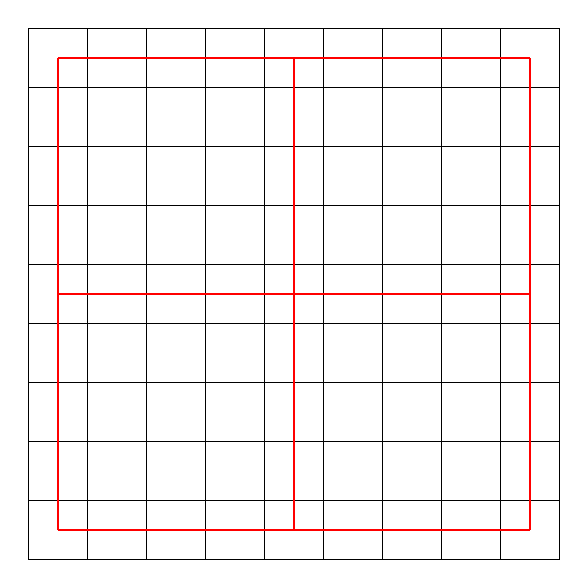
\begin{tikzpicture}[scale=0.75]
    \draw (0,0) grid (9,9);
    \draw[step=4,thick,xshift=0.5cm,yshift=0.5cm] [red] (0,0) grid (8,8);
  \end{tikzpicture}
  \caption{Расположение вершин квадродерева в параметрическом пространстве.}
  \label{fig:quadtree}
\endminipage\hfill
%
\minipage{0.45\textwidth}
  \centering
  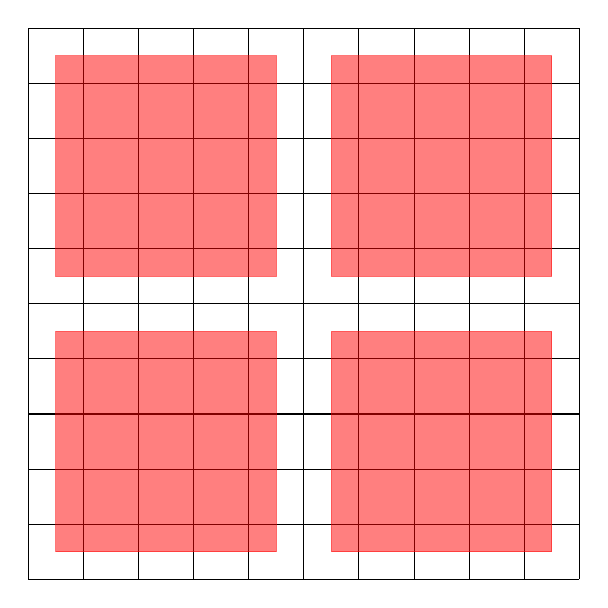
\begin{tikzpicture}[scale=0.7]
    \draw (0,0) grid (10,10);
    \filldraw [red, opacity=0.5, xshift=0.5cm,yshift=0.5cm]
      (0,0) rectangle (4,4)
      (0,5) rectangle (4,9)
      (5,0) rectangle (9,4)
      (5,5) rectangle (9,9);
  \end{tikzpicture}
  \caption{Области семплирования страниц в кэше }
  \label{fig:cache}
\endminipage
\end{figure}
Как было упомянуто выше, для мелкогранулярного выбора уровня детализации по модели данный алгоритм использует квадродеревья в рамках каждой карты. На каждом уровне дерева пространство параметризации делится на 4 равных квадрата. Из этого следует что граница разделения проходит по середине центрального пикселя геометрического изображения, соответственно новым вершинам дерева соответствуют регионы геометрического изображения пересекающиеся по центральным пикселям и имеют размер $2^{n-1} + 1$ (рисунок \ref{fig:quadtree}).

Для адаптации иерархии был выбран простейший алгоритм из \cite{niski2007multi} постепенно измельчающий разрез квадродерева в попытке сэкономить полигоны адаптируя части квадродерева по отдельности. Адаптация мип-уровня вершин квадродерева происходит посредством вычисления ограничивающей призмы, проецированием её в пространство камеры и поиском ограничивающего её прямоугольника. Логарифм корня площади этого прямоугольника в пикселях с учётом некоторой константы пропорциональности берётся за целевую плотность треугольников для данной вершины.


\subsubsection{Виртуализация}
Для виртуализации геометрических изображений был выбран простой алгоритм LRU-кэширования. Размер наименьшего мип-уровня $K$ берётся за размер страницы кэша, каждое геометрическое изображение разрезается на страницы с наложением в один пиксель (аналогично соответствию регионов пространства параметризации вершинам квадродерева), по мере нужды страницы соответствующих изображений загружаются в кэш хранимый на видеокарте (без наложения). Наличие отступа в полпикселя у каждой страницы с каждой стороны позволяет использовать билинейную фильтрацию для кэша без возникновения артефактов на границах. На рисунке \ref{fig:cache} красным обозначены сэмплируемые области страниц, интерполяция пикселей из разных страниц в остальной области не влияет на отображаемый результат.

Для вычисления позиции страницы определённого изображения $I$ на определённом мип-уровне $M$ в кэше используются таблицы индирекции. $I,M$-таблица имеет размер $2^{M - K}$ по высоте и ширине и в ячейках содержит либо номер ячейки в кэше содержащей соответствующую страницу, либо служебное значение $-1$, означающее что страница отсутствует в кэше.

Для стабилизации частоты кадров количество страниц, загружаемых за один кадр в кэш, ограничено. Из-за этого может возникать нужда в момент рендеринга получить данные из страницы не находящейся в данный момент в кэше. В таком случае вычисляется в какой странице мип-уровня на 1 меньше целевого находится текущая точка поверхности и повторяем процедуру лукапа страницы. Процесс повторяется пока не будет найдена доступная в кэше страница. Чтобы таковая всегда была, изображения наименьшего мип-уровня никогда не извлекаются из кэша. Таким образом не зависимо от состояния кэша всегда есть возможность отобразить модель в каком-то качестве, возможно меньшем чем желаемое.

Важным моментом является факт дублирования граничной информации страниц -- при вычислении элемента таблицы лукапа для точки параметрического пространства лежащей на границе между несколькими страницами можно выбрать любую из них. Однако неосторожная обработка этого момента может привести к разрывам. В данной работе всегда выбирается страница целиком лежащая в регионе текущей вершины атласа, а разрывы устраняются в рамках описанного ниже алгоритма.

\subsubsection{Устранение разрывов}
\begin{figure}[ht]
\minipage{0.45\textwidth}
  \centering
  \begin{tikzpicture}
    \draw[step=2] (0,0) grid (4,4);
    \draw[step=1] (4,0) grid (8,4);
    \filldraw[red] (4,1) circle (2pt);
    \filldraw[red] (4,3) circle (2pt);
    \node at (3.75,1) {А};
    \node at (3.75,3) {Б};
  \end{tikzpicture}
  \caption{Потенциальные разрывы}
  \label{fig:tearing}
\endminipage\hfill
%
\minipage{0.45\textwidth}
  \centering
  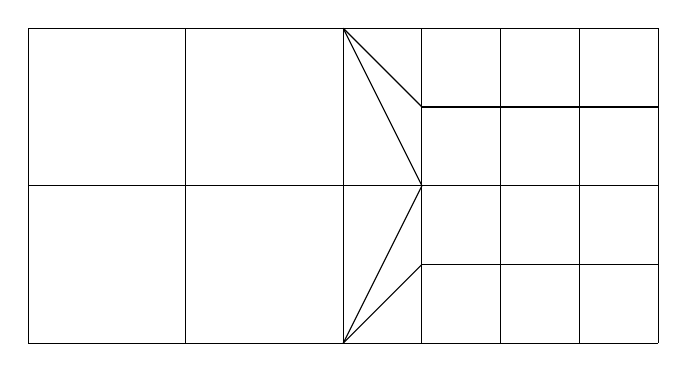
\begin{tikzpicture}
    \draw[step=2] (0,0) grid (4,4);
    \draw[step=1] (5,0) grid (8,4);
    \draw (4,0) -- (5,0);
    \draw (4,0) -- (5,1);
    \draw (4,0) -- (5,2);
    \draw (4,2) -- (5,2);
    \draw (4,4) -- (5,4);
    \draw (4,4) -- (5,3);
    \draw (4,4) -- (5,2);
  \end{tikzpicture}
  \caption{Устранение разрывов}
  \label{fig:stitching}
\endminipage
\end{figure}
При наивном рендеринге граничащих вершин квадродеревьев с разными мип-уровнями геометрических изображений будут образовываться разрывы из-за разной частоты дискретизации границы. На рисунке \ref{fig:tearing} вершины А и Б со стороны правой вершины могут не совпасть по координатам с серединой соответствующих рёбер левой вершины. Для устранения этой проблемы необходимо схлопывать рёбра со стороны вершины с б\'ольшим мип-уровнем согласно рисунку \ref{fig:stitching}. Однако может образовываться ситуация в которой вершина с высоким мип-уровнем граничит по одному ребру с несколькими вершинами различных более низких мип-уровней. В этой ситуации необходимо взять минимум из всех мип-уровней вершин опирающихся на это ребро и выбрать мип-уровень границы именно таким.

В данной работе используется следующий алгоритм поиска мип-уровней границ. Рассматриваются только вершины из активного среза. При изменении мип-уровня вершины перебрать все её рёбра, для каждого ребра найти всех опирающихся на него соседей и выбрать наибольшую по физическому размеру вершину. Для этой вершины находим всех соседей со стороны граничащей с изначальной вершиной, находим минимум из их мип-уровней и устанавливаем всем им мип-уровень границы на найденный минимум.

Для поиска соседних вершин входящих в срез, как отмечают в \cite{niski2007multi}, необходимо хранить в корнях деревьев 4 ссылки на соседние квадродеревья (их количество таково из свойств областей определений карт), а также ссылки на родителя в каждой вершине. Однако этой информации не достаточно. Как и при работе с обычными многообразиями, для переноса информации между различными картами необходимо иметь \emph{отображение склейки}, позволяющее отобразить параметрические координаты одной карты в параметрические координаты другой для точек лежащих в обоих картах. Для рассматриваемых нами атласов эти отображения всегда являются композицией переноса на целое число вдоль одной из осей и поворота на угол кратный $\frac{\pi}{2}$. Матрицы, задающие эти отображения, легко предподсчитываются сопоставлением координат вершин соответствующих углам геометрических изображений.

В данной работе дополнительно предподсчитываются для каждой вершины и каждой её стороны вершина, с которой достаточно начинать поиск соседей. В случае если с целевой стороны находится край текущей карты, этой вершиной является корень соседнего дерева. В ином случае такой вершиной служит первый из родителей текущей в порядке подъёма такой, что все вершины опирающиеся на грань текущей являются его потомками.

Наконец отметим, что при поиске мип-уровней границ необходимо учитывать в каком разрешении доступны страницы геометрического изображения на GPU на данном кадре. Для этого достаточно включать в поиск минимального мип-уровня для грани мип-уровни страниц, опирающихся на эту грань.

\subsubsection{Графический конвейер}
Для рендеринга иерархического атласа хорошо подходят тесселляционные шейдеры. Каждая модель рендерится при помощи одного вызова отрисовки с использованием инстансинга. Инстансы соответствуют выбранным вершинам квадродеревьев атласа, а количество вершин в каждом инстансе равно 4. Для каждого из них на видеокарту передаются выбранный мип-уровень, мип-уровни для сторон (именно за счёт них происходит описанное выше схлопывание), размер и позиция вершины в параметрическом пространстве, а также номер квадродерева, используя примитив данных ``patch list''. В вершинном шейдере по номеру вершины выбираются её координаты как одного из углов единичного квадрата. Далее шейдер управления тесселляцией выставляет режим ``quad'' и уровни тесселляции в соотетствии с мип-уровнями текущего инстанса. После тесселляции оценочный шейдер получает на вход одну из протесселлированных вершин расположенных равномерно (не считая границ) по единичному квадрату и используя их координаты, номер квадродерева и позицию в параметрическом пространстве вычисляет позицию вершины в параметрическом пространстве и обращаясь к соответствующей странице кэша по алгоритму, описанному выше, находит необходимые вершинные атрибуты, выставляет позицию вершины и передаёт остальные атрибуты во фрагментный шейдер для расчёта освещения.
